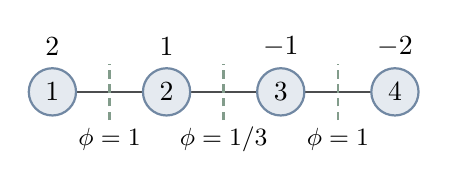
\begin{tikzpicture}[
  x=1.45cm,y=1cm,
  vertex/.style={circle,draw=graphSweepBlue,fill=graphSweepLight,
    line width=.8pt,minimum size=6mm,inner sep=0pt},
  cut/.style={draw=graphSweepGreen,densely dashed,line width=.85pt}
]
\definecolor{graphSweepBlue}{HTML}{7188A3}
\definecolor{graphSweepLight}{HTML}{E5EAF0}
\definecolor{graphSweepGreen}{HTML}{829C8B}
\definecolor{graphSweepLine}{HTML}{4C4D4F}
\draw[graphSweepLine,line width=.85pt] (0,0)--(3,0);
\foreach \i/\v/\f in {0/1/2,1/2/1,2/3/-1,3/4/-2}{
   \node[vertex] at (\i,0) {$\v$};
   \node at (\i,.57) {$\f$};
}
\foreach \i/\value in {.5/1,1.5/{1/3},2.5/1}{
   \draw[cut] (\i,-.36)--(\i,.35);
   \node[font=\small] at (\i,-.6) {$\phi=\value$};
}
\end{tikzpicture}
